\documentclass[12pt]{article}

% Packages
\usepackage[utf8]{inputenc}
\usepackage{amsmath, amssymb, amsthm}   % Math
\usepackage{graphicx}           % Images
% \usepackage{hyperref}           % Clickable links
\usepackage{geometry}           % Page margins
% \usepackage{cite}               % Citation formatting
\usepackage{algorithm}
\usepackage{algpseudocode}
\usepackage{listings}
\usepackage{color}

\definecolor{dkgreen}{rgb}{0,0.6,0}
\definecolor{gray}{rgb}{0.5,0.5,0.5}
\definecolor{mauve}{rgb}{0.58,0,0.82}

% BibLaTeX for references (requires biber)
\usepackage[
    backend=biber,
    style=numeric,
    sorting=nyt
]{biblatex}

\addbibresource{references.bib}  % Bib file

% Page setup
\geometry{margin=1in}

% Title
\title{Algorithms for efficient entropy conversion}
\author{Calum Grant \\
OxFORD Asset Management \\
calum.grant@oxam.com}
\date{\today}

\newtheorem{lemma}{Lemma}
\newtheorem{corollary}{Corollary}
\newtheorem{definition}{Definition}
\newtheorem{theorem}{Theorem}

\lstset{
  language=C,        % choose the language
  basicstyle=\ttfamily\small, % font style and size
  keywordstyle=\color{blue},
  commentstyle=\color{gray},
  stringstyle=\color{orange},
  numbers=left,
  numberstyle=\tiny\color{gray},
  stepnumber=1,
  numbersep=5pt,
  showstringspaces=false,
  breaklines=true,
  frame=single,
  captionpos=b
}

\begin{document}

\maketitle

\begin{abstract}
    We present new algorithms for converting random integers between different forms using an \em entropy store \em to cache entropy. The method can generate random variables for any weighted integer distribution, and consume entropy from any such distribution, whilst losing almost no entropy in the process.  For example we can shuffle a deck of 52 cards using just $\approxeq 225.58102$ bits of entropy, yielding an entropy conversion efficiency of $>0.99999992$ using a 32-bit entropy cache, compared with standard methods that only have a $\approxeq 0.81$ efficiency.  The algorithm requires two 32-bit integer divmod operations per random integer generated, making it significantly slower than other algorithms.
\end{abstract}

\section{Introduction}

In this paper, we will study the generation of perfectly distributed integers from an entropy source. A typical example of this is using fair coin flips to roll a fair die or to perform a perfect shuffle of a deck of cards, but there are practical applications of this such as XX.

The general problem is one of \em entropy conversion \em, where entropy in one form needs to be converted to entropy in a different form using a function $f$ on a discrete random variable $X$ having Shannon entropy $H(X)$.  A fundamental result is that you cannot get more entropy out than you put in, or $H(X) \ge H(f(X))$ \ref{entropy}. We will be primarily focussed on improving the efficiency of entropy conversion, defined as $\eta = \frac{H(f(X))}{H(X)}$.

Whilst this problem has been studied extensively, there are theoretical limits when generating integers one at a time, because algorithms must always fetch entropy in units. In fact we must fetch up to 2 extra bits of entropy per integer generated \ref{xx}.  For example to roll a fair d6 die requires $\frac{11}{3} \approxeq 3.6$ coin flips on average, but the entropy contained in the d6 is $\log_26 \approxeq 2.58$. When shuffling a deck of 52 cards, fetching integers one at a time requires $\approxeq 278$ bits of entropy to perform the shuffle, against an output entropy of $\log_252! \approxeq 225.58$.

To mitigate these entropy losses, it's possible to generate random integers in batches. The major drawback with existing batching schemes is that they are somewhat complex and expensive to implement, or require you to know beforehand which numbers you need to generate. Whilst they improve entropy efficiency they still compromise on performance and efficiency.

In this paper we will explore a fundamentally different approach. We will allow every entropy conversion algorithm to have access to an \em entropy store \em in the form of a large uniformly distributed integer (of the order of 32 bits), and allow the algorithm to put back any unused entropy into the store. By carefully analysing the steps that could lose entropy, we can reclaim nearly all lost entropy, giving a near-perfect entropy conversion efficiency. 

The entropy efficiency depends only on the ratio of the size of the store $N$ to the size $n$ of the number generated, and a precise bound is calculated in Theorem \ref{xx}. For example to roll a 6-sided die with a 32-bit entropy store ($N\ge2^{31}$) has an entropy efficiency of $>0.99999997$ To shuffle a deck of 52 cards with a 32-bit entropy store has an entropy efficiency $>0.99999992$. By increasing the size of the store, we can achieve entropy efficiency arbitrarily close to 1.

The algorithms are easy to implement, require O(1) time and memory, and use two integer divmod operations per uniform integer generated. To convert between distributions, and additional $O(n)$ of lookup tables is required. The main benefit of these algorithms is their simplicity, flexibility and high efficiency.

\subsection {Contribution}

\section{Related work}


\section{Algorithms for entropy conversion}

\subsection{Fundamental operations}

In this section we'll start with some basic operations (Algorithm \ref{alg:combine}-\ref{alg:upsample}), then use these to create an efficient generator for uniform integers (Algorithm \ref{alg:generate-uniform}) using an entropy store.

We'll then build on Algorithm \ref{alg:generate-uniform} to create a generator for an arbitrary weighted distribution (Algorithm \ref{alg:generate-distribution}), extract entropy from a weighted distribution (Algorithm \ref{alg:combine-distribution}), and use these to convert entropy between arbitrary distributions (Algorithm \ref{alg:convert-distribution}). All of these algorithms are designed to have a 1 or near-1 entropy efficiency, and proofs of correctness and efficiency are contained throughout this section.

Algorithm \ref{alg:combine} combines entropy from two uniform distrete random variables into a single uniform random variable.

\begin{algorithm}
\caption{Combining uniformly distributed integers}
\label{alg:combine}
\begin{algorithmic}[1]
    \Require $n$, $m$, $U_n$, $U_m$ are integers
    \Require $n>0$, $m>0$
    \Require $U_n$ is uniformly distributed over $[0,n)$
    \Require $U_m$ is uniformly distributed over $[0,m)$
    \Ensure $nm$ is $n * m$
    \Ensure $U_{nm}$ is uniformly distributed over $[0,nm)$
\Procedure{combine}{$U_n, n, U_m, m$} 
  \State $U_{nm} \gets U_n * m + U_m$
  \State $nm \gets n * m$
  \State \Return $U_{nm}, nm$
\EndProcedure
\end{algorithmic}
\end{algorithm}

\begin{lemma}
In Algorithm \ref{alg:combine}, $U_{nm}$ is uniformly distributed over $[0,nm)$.
\label{lem:combine}
\end{lemma}

\begin{proof}
Let $X \sim Uniform \{0 ... n-1\}$ and $Y \sim Uniform\{0 ... m-1\}$ be independent uniformly distributed random variables. The joint distribution $(X,Y)$ is uniformly distributed with $nm$ elements of probability $\frac{1}{nm}$. Let $Z$ be the distribution defined as

\begin{equation}
Z = f(X,Y) = mX+Y
\end{equation}

The mapping $f$ is a bijection between the pair $X \times Y$ and $Z$, so $Z$ is also uniformly distributed and 

\begin{equation}
Z \sim Uniform \{0 ... nm-1\}
\end{equation}
\end{proof}

Algorithm \ref{alg:divide} is the inverse of Algorithm \ref{alg:combine}, allowing us to factorise a uniformly distributed integer into two. For this, the sizes of the output distributions must divide the size of the input distribution.

\begin{algorithm}
\caption{Division of uniformly distributed integers}
\label{alg:divide}
\begin{algorithmic}[1]
    \Require $nm$, $n$, $U_{nm}$ are integers
    \Require $nm>0$, $m>0$
    \Require $nm$ is divisible by $n$
    \Require $U_{mn}$ is uniformly distributed over $[0,nm)$
    \Ensure $n * m = nm$
    \Ensure $U_{n}$ is uniformly distributed over $[0,n)$
    \Ensure $U_{m}$ is uniformly distributed over $[0,m)$
    \Ensure $U_n$ and $U_m$ are independent
\Procedure{divide}{$U_{nm}, mn, n$} 
  \State $U_m \gets U_{nm} \operatorname{div} n$
  \State $U_{n} \gets U_{nm} \mod n$
  \State $m \gets nm / n$
  \State \Return $U_n, U_m, m$
\EndProcedure
\end{algorithmic}
\end{algorithm}

\begin{lemma}
In Algorithm \ref{alg:divide}, $U_n$ is uniformly distributed over $[0,n)$ and $U_m$ is uniformly distributed over $[0,m)$. $U_m$ and $U_n$ are independent.

\label{lem:divide}
\end{lemma}

\begin{proof} $f$ is a bijection so has an inverse function 
\begin{equation}    
X = \lfloor Z/n \rfloor, Y = Z \mod n
\end{equation}

Since $X$ and $Y$ are the original random variables, they are independent and uniformly distributed.
\end{proof}

Algorithm \ref{alg:downsample} converts a uniformly distributed integer to a smaller range, and also returns a biassed bit. Unlike Algorithm \ref{alg:combine} and Algorithm \ref{alg:divide}, the size of the output distribution depends on the value. The biassed bit also contains entropy, and in fact the total entropy returned by this algorithm is the same as its input entropy.

\begin{algorithm}
\caption{Downsampling uniformly distributed integers}
\label{alg:downsample}
\begin{algorithmic}[1]
    \Require $U_{n}$, $m$ and $n$ are integers 
    \Require $0 \le m \le n$
    \Require $U_{n}$ is uniformly distributed over $[0,n)$
\Ensure $U_{x}$ is uniformly distributed over $[0,x)$
\Ensure $x = m$ or $x=n-m$
\Ensure $B$ is a Boolean value Bernoulli distributed with $p=\frac{m}{n}$
\Ensure $U_x$ and $B$ are independent
\Procedure{downsample}{$U_n, n, m$} 
  \If{$U_n < n$}
    \State $B \gets True$  
    \State $x \gets m$
    \State $U_x \gets U_n$
  \Else
    \State $B \gets False$  
    \State $x \gets m-n$
    \State $U_x \gets U_n-m$
  \EndIf
  \State \Return $U_x, x, B$
\EndProcedure
\end{algorithmic}
\end{algorithm}

\begin{lemma}
In Algorithm \ref{alg:downsample}, $U_x$ is uniformly distributed over $[0,x)$.
\label{lem:downsample}
\end{lemma}

\begin{proof}
    Let $y = U_n$.
    $P(y<m) = \frac{m}{n}$ so $B \sim Bernoulli\{\frac{m}{n}\}$.

If $y < m$, then $y$ is uniformly distributed between $[0,m)$.

If $y \ge m$, then $y$ is uniformly distributed between $[m, n)$, so $y-m$ is uniformly distributed between $[0, n-m)$.
\end{proof}

Algorithm \ref{alg:upsample} increases the size of a uniform distribution by incorporating Bernoulli entropy. This could be used to harness entropy from biassed Bernoulli sources.

\begin{algorithm}
\caption{Upsampling uniformly distributed integers}
\label{alg:upsample}
\begin{algorithmic}[1]
\Require $U_x$ is uniformly distributed over $[0,x)$
\Require $B$ is a Boolean value Bernoulli distributed with $p=\frac{m}{n}$
\Require $x=m$ if $B$ else $x=n-m$
\Ensure $U_n$ is uniformly distributed over $[0,n)$.
\Procedure{upsample}{$U_x, x, n, B$} 
  \If{$B$}
    \State $U_n \gets U_x$  
  \Else
    \State $U_n \gets n-x+U_x$  
  \EndIf
  \State \Return $U_n$
\EndProcedure
\end{algorithmic}
\end{algorithm}

\begin{lemma}
In Algorithm \ref{alg:upsample}, $U_{n}$ is uniformly distributed over $[0,n)$.
\end{lemma}

\begin{proof}
Let $x = U_{n} \sim X$. The possible values of $X$ are $\{0 ... n-1\}$.

Case 1: $x<n$

\begin{align}
P(x=X) & = P(B)P(x=X|B) + P(\neg B)P(x=X|\neg B) \\
       & = \frac{m}{n}\frac{1}{m} + 0 \\
       & = \frac{1}{n}
\end{align}

Case 2: $x \ge n$

\begin{align}
P(x=X) & = P(B)P(x=X|B) + P(\neg B)P(x=X|\neg B) \\
       & = 0 + (1 - \frac{m}{n})\frac{1}{n-m}  \\
       & = \frac{n - m}{n}\frac{1}{n-m} \\
       & = \frac{1}{n}
\end{align}

This means that $x \sim Uniform\{0...n-1\}$.
\end{proof}

\subsection{Generating uniform integers}

Algorithm \ref{alg:generate-uniform} reads binary entropy from a $fetch()$ function, and outputs a uniform integer in the range $[0,n)$. The algorithm makes use of an \em entropy store \em $U_s$ which is carried over in between function calls. In a practial implementation, $U_s$ and $s$ can be captured variables or class members. Initially the entropy store is empty (containing $0$ entropy) with $U_s = 0$ and $s=1$.

The overall strategy of Algorithm \ref{alg:generate-uniform} is to use $downsample$ (Algorithm \ref{alg:downsample}) to ensure that $s$ is a multiple of $n$, then use the $divide$ algorithm (Algorithm \ref{alg:divide}) to divide $U_s$ into $U_n$. $U_n$ is returned as the result, and $U_s$ which is stored for the next invocation. The calculation is structured so that when $s$ is large, the entropy lost by $downsample$ is very small.

The $downsample$ on line 6 resizes $s$ to a multiple of $n$. It is overwhelmingly likely that $b$ is false because $n$ is much smaller than $s$, so we can then proceed to line 8 where we divide $U_s$ into $U_n$ and the new $U_s$. On line 9, return $U_n$ as the result and $U_s$ and $s$ as the input to the next invocation.

An C implemetation of Algorithm \ref{alg:generate-uniform} is given in Appendix \ref{adx:source}.

\begin{algorithm}
\caption{Generating uniformly distributed integers}
\label{alg:generate-uniform}
\begin{algorithmic}[1]
\Require Integers $0 < n\le N$
\Require $fetch()$ returns Bernoulli entropy with $p=0.5$
\Require $U_s$ is uniformly distributed over $[0,s)$
\Ensure $U_n$ is uniformly distributed over $[0,n)$
\Ensure $U_s$ is uniformly distributed over $[0,s)$
\Procedure{generate\_uniform}{$U_s, s, n, N$} 
  \While {True}
    \While {$s < N$}
        \State $U_s, s \gets combine(U_s, s, fetch(), 2)$
    \EndWhile
    \State $U_s, s, b \gets downsample(U_s, s, s \mod n)$ 
    \If{$ \neg b$}
        \State $U_n, U_s, s \gets divide(U_s, s, n)$
        \State \Return $U_s, s, U_n$
    \EndIf
  \EndWhile
\EndProcedure
\end{algorithmic}
\end{algorithm}

\begin{lemma}
    In Algorithm \ref{alg:generate-uniform}, 
$U_n$ is uniformly distributed over $[0,n)$ and 
$U_s$ is uniformly distributed over $[0,s)$.
\end{lemma}

\begin{proof}
The values $U_n$, $n$, $U_s$ and $s$ have been generated by Algorithms \ref{alg:combine}, \ref{alg:divide} and \ref{alg:downsample}. By Lemmas \ref{lem:combine}, \ref{lem:divide} and \ref{lem:downsample}, $U_n$ and $U_s$ are uniformly distributed.
\end{proof}

\begin{lemma}
Algorithm \ref{alg:generate-uniform} terminates with probability 1.
\end{lemma}

\begin{proof}
    If $p$ be the probability that the algorithm loops, where $p<1$, then the probability $q$ that Algorithm \ref{alg:generate-uniform} loops forever is given by $q = (1-p)q \implies q=0$.
\end{proof}

\subsection{Generating weighted integer distributions}

Algorithm \ref{alg:generate-distribution} shows how we can generate an arbitrary  distribution of $k$ outcomes where each outcome has integer weight ${w_1 ... w_k}$, normalised to a discrete distribution with probabilities $\{\frac{w_1}{n}, \frac{w_2}{n} ... \frac{w_k}{n}\}$ where $n=\sum_i w_i$ is the total weight.

The algorithm works by construct an injective mapping from the $n$ outcomes of a uniform distribution to the $k$ outputs of the weighted distribution. This is a simple lookup table of size $n$. If $n$ is very large we'll need to implement this differently.

To generate an output, call $generate\_uniform$ to generate a integer in the range $[0,n)$, and use the number in the lookup table as the result. 

Notice though that we also can generate a uniform distribution of size $w_i$, due to the index of $n$ within each output range. Figure \ref{fig:bins} illustrates this. When we perform a multi-way downsample, the output is a distribution $X$ and a uniform distribution $Y \sim Uniform [0,w_i)$. $Y$ is uniformly distributed because it is drawn from a uniform distribution.

% Figure bin: 

Lemma \ref{lem:distribution-conservation} shows us that when we account for this extra entropy in $Y$ then no entropy is lost. So the final step in Algorithm \ref{alg:generate-distribution} is to capture the extra entropy from the uniform distribution $Y$ back into the entropy store.

\begin{lemma}
    \label{lem:distribution-conservation}
    When we downsample $Uniform\{0..n-1\}$ into weighted distribution $X$ and $Y \sim Uniform\{0,w_i-1\}$, entropy is conserved.
\end{lemma}

\begin{proof}
    \begin{align}
    E(H_{lhs}) & = \log_2 n \\
    E(H_{rhs}) & = E(H(X)) + E(H(Y)) \\ 
               & = - \sum_i p_i \log_2p_i + \sum_i p_iH(Y|X=i) \\
               & = - \sum_i \frac{w_i}{n} \log_2 \frac{w_i}{n} + \sum_i \frac{w_i}{n}\log_2 w_i \\
               & = - \sum_i \frac{w_i}{n}(\log_2 w_i - \log_2 n) + \sum_i \frac{w_i}{n}\log_2 w_i \\
               & = - \sum_i \frac{w_i}{n}\log_2 w_i + \sum_i \frac{w_i}{n} \log_2 n + \sum_i \frac{w_i}{n}\log_2 w_i \\
               & = \sum_i \frac{w_i}{n} \log_2 n \\
               & = \frac{\log_2 n}{n} \sum_i w_i \\
               & = \frac{\log_2 n}{n} n \\
               & = \log_2 n
    \end{align}
\end{proof}

\begin{algorithm}
\caption{Constructing lookup tables for a weighted random variable}
\label{alg:generate-lookup-tables}
\begin{algorithmic}[1]
\Require $weights$ is a list of integers $\ge0$
\Procedure{make\_distribution}{$weights$} 
  \State $outputs \gets []$
  \State $offsets \gets []$
  \For {$w_i \in weights$}
    \State $offsets \gets offsets + [|outputs|]$
    \State $outputs \gets outputs + [i] * w_i$
  \EndFor
  \State \Return $outputs, offsets$
\EndProcedure
\end{algorithmic}
\end{algorithm}


\begin{algorithm}
\caption{Generating a weighted random variable}
\label{alg:generate-distribution}
\begin{algorithmic}[1]
\Require $U_s$, $s$, $N$ are integers
\Require $weights$ is an array of integers $w_i \ge 0$
\Require $offset$ generated by $make\_distribution$ 
\Require $outputs$ generated by $make\_distribution$
\Require $U_s$ is uniformly distributed over $[0,s)$
\Require $N >> |outputs|$
\Ensure $U_s$ is uniformly distributed over $[0,s)$
\Procedure{generate\_distribution}{$U_s, s, N, weights, outputs, offsets$} 
    \State $n \gets |outputs|$
    \State $U_s, s, U_n \gets generate\_uniform(U_s, s, N, n)$
    \State $U_s, s = combine(U_s, s, U_n - offsets[U_n], weights[outputs[U_n]])$
    \State \Return $U_s, s, outputs[U_n]$
\EndProcedure
\end{algorithmic}
\end{algorithm}

Algorithm \ref{alg:combine-distribution} performs the inverse of Algorithm \ref{alg:generate-distribution}. It reconstructs a uniform distribution of size $n$ from the weighted distribution variable, and combines it with a uniform distribution of size $w_i$. This allows the entropy store to absorb the entropy from $i$.

Note that when performing the inverse of Algorithm \ref{alg:generate-distribution}, we don't need to supply it the *same* random variable $U_x$ that was originally used, and we can just get one from our entropy store.

We'll ignore potential integer overflows of $U_s$ and $s$.

\begin{algorithm}
\caption{Extracting entropy from a weighted random variable}
\label{alg:combine-distribution}
\begin{algorithmic}[1]
\Require $U_s$, $s$, $N$ are integers
\Require $weights$ is an array of integers $w_i \ge 0$
\Require $offset$ generated by $make\_distribution$ 
\Require $outputs$ generated by $make\_distribution$
\Require $U_s$ is uniformly distributed over $[0,s)$
\Require $N >> |outputs|$
\Ensure $U_s$ is uniformly distributed over $[0,s)$
\Procedure{combine\_distribution}{$U_s, s, N, weights, outputs, offsets, i$} 
    \State $U_s, s, U_x \gets generate\_uniform(U_s, s, N, weights[i])$
    \State $U_s, s \gets combine(U_s, s, U_x + offsets[i], |outputs|)$
    \State \Return $U_s, s$
\EndProcedure
\end{algorithmic}
\end{algorithm}

Finally we can compose Algorithm \ref{alg:generate-distribution} and Algorithm \ref{alg:combine-distribution} into a single step in Algorithm \ref{alg:convert-distribution}. This allows entropy to be converted from one form to another via the entropy store.


\begin{algorithm}
\caption{Converting entropy between weighted random variables}
\label{alg:convert-distribution}
\begin{algorithmic}[1]
\Require $U_s$, $s$, $N$ are integers
\Require $W_{in}$ is an array of integers $w_i \ge 0$
\Require $O_{in}$ generated by $make\_distribution$ 
\Require $T_{in}$ generated by $make\_distribution$
\Require $U_s$ is uniformly distributed over $[0,s)$
\Require $N >> |outputs|$ TODO
\Require $i$ is distributed fairly according to $W_{in}$, $O_{in}$ and $T_{in}$
\Ensure $j$ is distributed fairly according to $W_{in}$, $O_{in}$ and $T_{in}$
\Ensure $U_s$ is uniformly distributed over $[0,s)$
\Procedure{convert\_distribution}{$U_s, s, N, W_{in}, O_{in}, T_{in}, W_{out}, O_{out}, T_{out}, i$} 
    \State $U_s, s \gets combine\_distribution(U_s, s, N, W_{in}, I_{in}, T_{in}, i)$
    \State $U_s, s, j \gets generate\_distribution(U_s, s, N, W_{out}, O_{out}, T_{out})$
    \State \Return $U_s, s, j$
\EndProcedure
\end{algorithmic}
\end{algorithm}


\section {Efficiency of entropy conversion algorithms}

In this section we'll calculate bounds on the entropy efficiency of Algortithms \ref{alg:combine}-\ref{alg:convert-distribution}, and prove that these algorithms have entropy efficiency 1 or arbitrarily close to 1.

Insert notation here.

\begin{lemma}
\label{lem:conservation}
Algorithms \ref{alg:combine}-\ref{alg:upsample} conserve entropy.
\end{lemma}

\begin{proof}
We can calculate the before and after entropy for each of these algorithms to see that they are the same. But we can also observe that since each algorithm has an inverse (Algorithm \ref{alg:combine} inverts Algorithm \ref{alg:divide}; Algorithm \ref{alg:upsample} inverts Algorithm \ref{alg:downsample}), entropy must be conserved.
\end{proof}

The \em rejection sampling \em algorithm (Algorithm \ref{alg:rejection-sampling}), and Fast Dice Roller (Algorithm \ref{alg:fast-dice-roller}) use a form of Algorithm \ref{alg:downsample}, but do lose entropy because they throw away the $B$ term. The entropy of the internal decision is exactly the entropy that is lost by these algorithms.

\begin{lemma}
    \label{lem:shannon-inequality}

For $p,q \in \mathbb{R}$, where $0 \le p\le q \le 0.5$, 

\begin{equation}
-p\log_2 p - (1-p)\log_2(1-p) \le -q\log_2 q - (1-q)\log_2(1-q)
\end{equation}
\end{lemma}

\begin{proof}
    Let
    \begin{align}
        g(p) & = -p\log_2 p - (1-p)\log_2(1-p) \\
        \implies g'(p) & = \log_2\frac{1-p}{p} = \log_2(\frac{1}{p}-1) \ge \log_21 = 0 
    \end{align}
Since the derivative of $g>0$ it means that $g$ is monotonic.
\end{proof}

\begin{definition}
    Let $H_{loss}(p)$ be the expected entropy loss function of Algorithm \ref{alg:generate-uniform}, for $p=\frac{n-1}{N}$.
\end{definition}

\begin{theorem}
    \label{thm:loss}
If $p = \frac{n-1}{N} < 0.5$,

\begin{equation}
0 \le H_{loss}(p) \le -\frac{p}{1-p}\log_2p - \log_2(1-p)
\end{equation}

\end{theorem}

\begin{proof}
For each iteration $i$ of Algorithm \ref{alg:generate-uniform}, let $p_i = \frac{s_i \mod n}{s_i}$. But $(s_i \mod n) \le n-1$ and $s_i \ge N$, so $\frac{s_i \mod n}{s_i} \le \frac{n-1}{N}$, so $p_i \le p$. On each iteration, the entropy lost is equal to the entropy in the variable $b_i \sim Bernoulli\{p_i\}$, which is given by the entropy equation for a Bernoulli distribution \ref{todo}:

\begin{equation}
H(b_i) = -p_i\log_2p_i - (1-p_i)\log_2(1-p_i)
\end{equation}

Therefore, 

\begin{equation}
0 \le H(b_i) \le -p\log_2p - (1-p)\log_2(1-p) 
\end{equation}


by Lemma \ref{lem:shannon-inequality}. The expected number of iterations $N$ is given by

\begin{align}
& N = 1 + p_iN \le 1 + pN \\
\implies & N-pN \le 1 \\
\implies & N(1-p) \le 1 \\
\implies & N \le \frac{1}{1-p}
\end{align}

The total entropy lost by the algorithm is given by the number of iterations of the algorithm multiplied by the entropy lost in each iteration.

\begin{align}
0 \le NH(b_i) \le & \frac{1}{1-p}(-p\log_2p - (1-p)\log_2(1-p) ) \\
= & -\frac{p}{1-p}\log_2p - \log_2(1-p)
\end{align}

We can also end up in the situation where $(s \mod n) = 0$ already, in which the \em downsample \em step always succeeds with no entropy loss, so $H_{loss}=0$.
\end{proof}

The actual entropy loss incurred by Algorithm \ref{alg:generate-uniform} depends on whatever values are found in $U_s$ and $s$, so we can only give an upper bound.

\begin{corollary}
The entropy efficiency $\eta$ of Algorithm \ref{alg:generate-uniform} is bounded by

\begin{equation}
\frac{\log_2n}{\log_2n + H_{loss}(\frac{n-1}{N})} \le \eta \le 1
\label{eq:generate-uniform-efficiency}
\end{equation}
\end{corollary}

\begin{proof}
\begin{align}
    \eta & = \frac{H_{out}}{H_{in}} \\
         & = \frac{H_{out}}{H_{out}+H_{loss}} \\
         & = \frac{\log_2n}{\log_2n + H_{loss}(\frac{n-1}{N})}
\end{align}
Therefore 
\begin{equation}
\frac{\log_2n}{\log_2n + H_{loss}(\frac{n-1}{N})} \le \eta \le 1
\end{equation}
from Theorem \ref{thm:loss}.
\end{proof}

To illustrate Equation \ref{eq:generate-uniform-efficiency}, if $N=2^{31}$ and $n=6$, then $\eta \ge 0.99999997$. This means that even with a modest entropy buffer, we can get very good entropy efficiency.

\begin{corollary}
The entropy efficiency $\eta$ of Algorithm \ref{alg:generate-uniform} is arbitrarily close to 1.
\end{corollary}

\begin{proof}
$H_{loss}(\frac{n-1}{N}) \rightarrow 0$ as $N \rightarrow \infty$. Therefore $\eta \rightarrow 1$ as $N \rightarrow \infty$.
\end{proof}


\begin{corollary}
The entropy loss of Algorithm \ref{alg:convert_u_u} is $H_{loss}(\frac{n-1}{N})$.
\end{corollary}

\begin{proof}
    Algorithm \ref{alg:convert_u_u} only loses entropy through $generate\_uniform$ which loses $H_{loss}(\frac{n-1}{N})$. The $combine$ operation does not lose entropy by Lemma \ref{lem:conservation}.
\end{proof}

\begin{corollary}
The entropy loss of Algorithm \ref{alg:generate-bernoulli} is given by $H_{loss}(\frac{n-1}{N})$.
\end{corollary}

\begin{proof}
    Algorithm \ref{alg:generate-bernoulli} only loses entropy through $generate\_uniform$ which loses $H_{loss}(n)$. The $downsample$ $combine$ operations do not lose entropy by Lemma \ref{lem:conservation}.
\end{proof}

\begin{lemma}
    \label{lem:hloss_monotonic}
    $H_{loss}(p)$ is monotonically increasing in the range $0 < p < 1$.
\end{lemma}

\begin{proof}The derivative of $H_{loss}$ is
    \begin{equation}
        \frac{-\log_2p}{(1-p)^2}
    \end{equation}
    which is positive in the range $0 < p < 1$.
\end{proof}

\begin{lemma}
The entropy loss of Algorithm \ref{alg:consume_b} is no more than than $H_{loss}(\frac{n-1}{N})$
\end{lemma}

\begin{proof}
    The entropy-losing step in Algorithm \ref{alg:consume_b} is $generate\_uniform$ which loses $H_{loss}(\frac{x-1}{N})$ bits. $x \le n$, so from Lemma \ref{lem:hloss_monotonic}, this means that $H_{loss}(\frac{x-1}{N}) \le H_{loss}(\frac{n-1}{N})$.
\end{proof}

\begin{corollary}
The amortised entropy lost by Algorithm \ref{alg:convert_b_b} is no more than $H_{loss}(\frac{n_1-1}{N}) + H_{loss}(\frac{n_2-1}{N})$
\end{corollary}

\begin{proof}
    $consume\_bit$ loses $H_{loss}(\frac{n_1-1}{N})$ bits of entropy, and $generate\_bit$ loses $H_{loss}(\frac{n_2-1}{N})$ bits of entropy.
\end{proof}









\section {Evaluation}


In terms of time, all EEC algorithms are O(1). On modern CPUs, the most expensive operation is integer division, which is usually as expensive as divide and modulus (divmod) \cite{cpudivmod}. This makes the $divide$ algorithm (Algorithm \ref{alg:divide}) the most expensive algorithm using two integer divisions, but it is still O(1).




We can compare the entropy efficiency of different algorithms. Backer et al [] compared the efficiency of random integer generation of rejection sampling (Algorithm \ref{alg:rejection-sampling}) and Knuth-Yau, implemented as Lombraso's Fast Dice Roller algorithm (Algorithm \ref{alg:fast-dice-roller}). To this comparison we can now add Algorithm \ref{alg:generate-uniform}.

Figure \ref{fig:uniform} shows the entropy efficiency when generating a single integer in the range $[0,n)$.  Algorithms that do not store entropy are much less efficient, and as observed by Backer et al \cite{todo}, the efficiency depends on the number being generated. For Algorithm \ref{alg:generate-uniform}, efficiency does decrease with the number generated according to Equation \ref{eq:generate-uniform-efficiency}, but it is not visible on this graph.

\begin{figure}[ht]
\centering
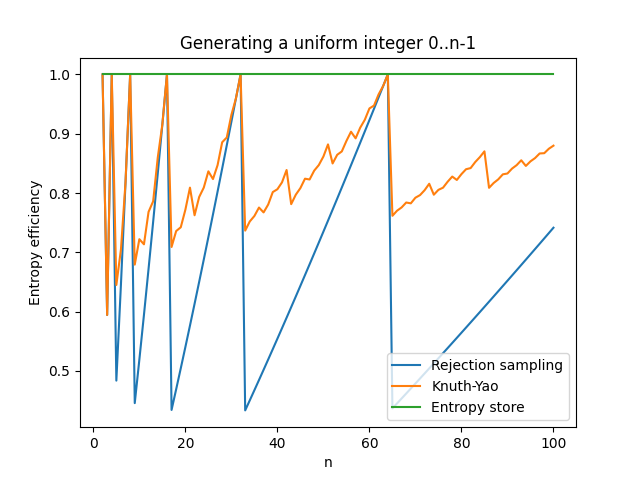
\includegraphics[width=0.5\textwidth]{uniform_efficiency.png}
\caption{Entropy efficiency for uniform integer generation.}
\label{fig:uniform}
\end{figure}

Figure \ref{fig:shuffle} shows the entropy efficiency when shuffling a deck of $n$ cards using the Fisher-Yates algorithm \cite{fisher-yates}.

\begin{figure}[ht]
\centering
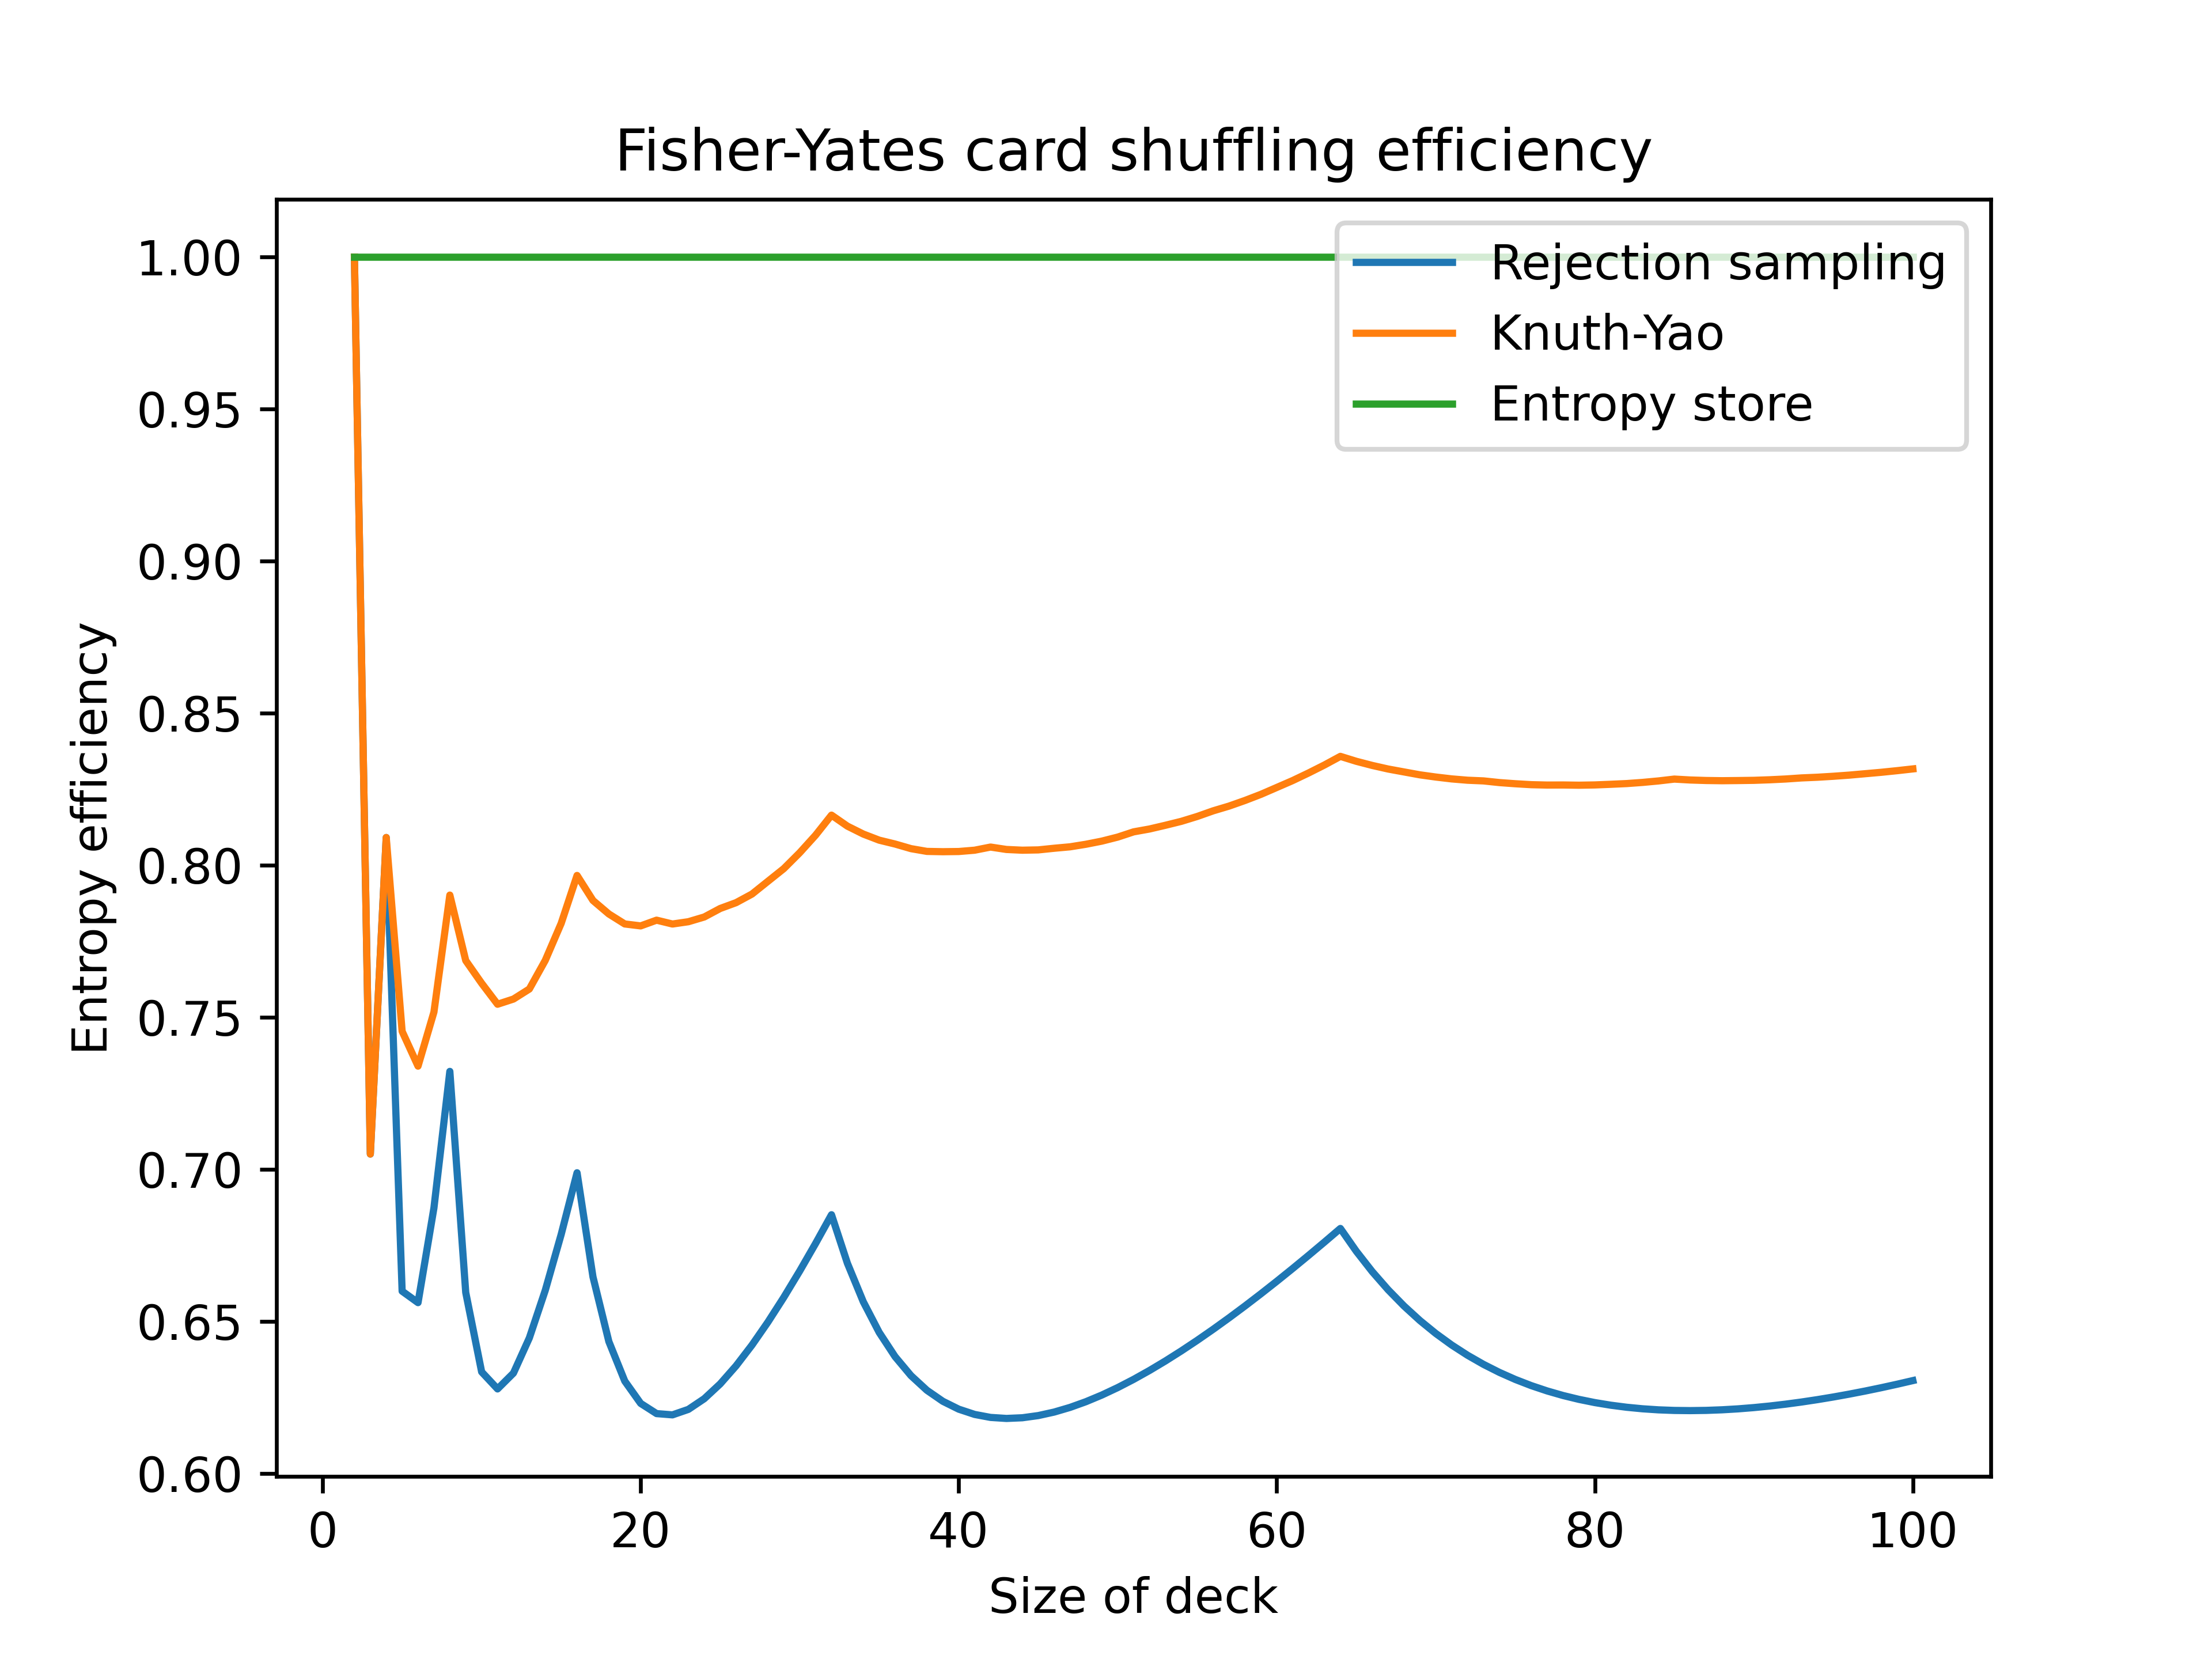
\includegraphics[width=0.5\textwidth]{shuffling_efficiency.png}
\caption{Entropy efficiency for card shuffling.}
\label{fig:shuffle}
\end{figure}






\section{Discussion}





\section{Conclusion}

We showed that entropy can be converted between different forms much more efficiently if we are able to pre-fetch and store entropy between invocations. Then we can exploit the large value in the entropy store to make an extremely asymmetrical descision that loses a minimum of entropy.

We have shown that the amortised entropy conversion efficiency can be arbitrarily close to 1, and the efficiency depends on the the size of the entropy store relative to the integer being generated. For applications like dice-rolling or card-shuffling, we can store the entropy in a 32-bit integer and can achieve an amortised entropy efficiency of $> 0.999999924$.

As well a generating uniform integers, we can read and generate entropy values $<1$ in the form of Bernoulli entropy, with near 1 efficiency.

This can have practical applications where the numbers generated must genuinely random and not from a pseudo-random number generator.

\printbibliography

\section {Appendix A}
Here is the source code for $generate\_uniform$, written in C.

\begin{verbatim}
    static const uint32_t N = 1<<31;
    uint32_t s_value = 0, s_range = 1;

    uint32_t generate_uniform(uint32_t n)
    {
        for(;;)
        {
            // Preload entropy one bit at a time into s
            while(s_range < N)
            {
                s_value <<= 1;
                s_value |= fetch();
                s_range <<= 1;
            }
            // Resample entropy s to a multiple of n
            uint32_t r = s_range / n;
            uint32_t c = s_range % n;
            if(s_value >= c)
            {
                // Resample successful
                s_value -= c;
                uint32_t a = s_value / n;
                uint32_t b = s_value % n;
                s_value = a;
                s_range = r; 
                return b;
            }
            else
            {
                // Resample unsuccessful
                s_range = c;
            }
        }
    }
\end{verbatim}

\end{document}
